\documentclass[tikz,border=10pt]{article}
\usepackage[paperwidth=34cm,paperheight=16cm,margin=0.3cm]{geometry}
\usepackage{tikz}
\usetikzlibrary{arrows.meta, calc, decorations.pathreplacing, patterns}
\pagestyle{empty}

\definecolor{audioblue}{HTML}{2A6FDB}
\definecolor{crossfadeamber}{HTML}{E8A838}
\definecolor{gengreen}{HTML}{2EAA4F}
\definecolor{llmred}{HTML}{E05555}
\definecolor{updateorange}{HTML}{E07B39}
\definecolor{waitgray}{HTML}{AAAAAA}
\definecolor{promptgray}{HTML}{555555}
\definecolor{timegray}{HTML}{888888}
\definecolor{axisgray}{HTML}{BBBBBB}

\begin{document}
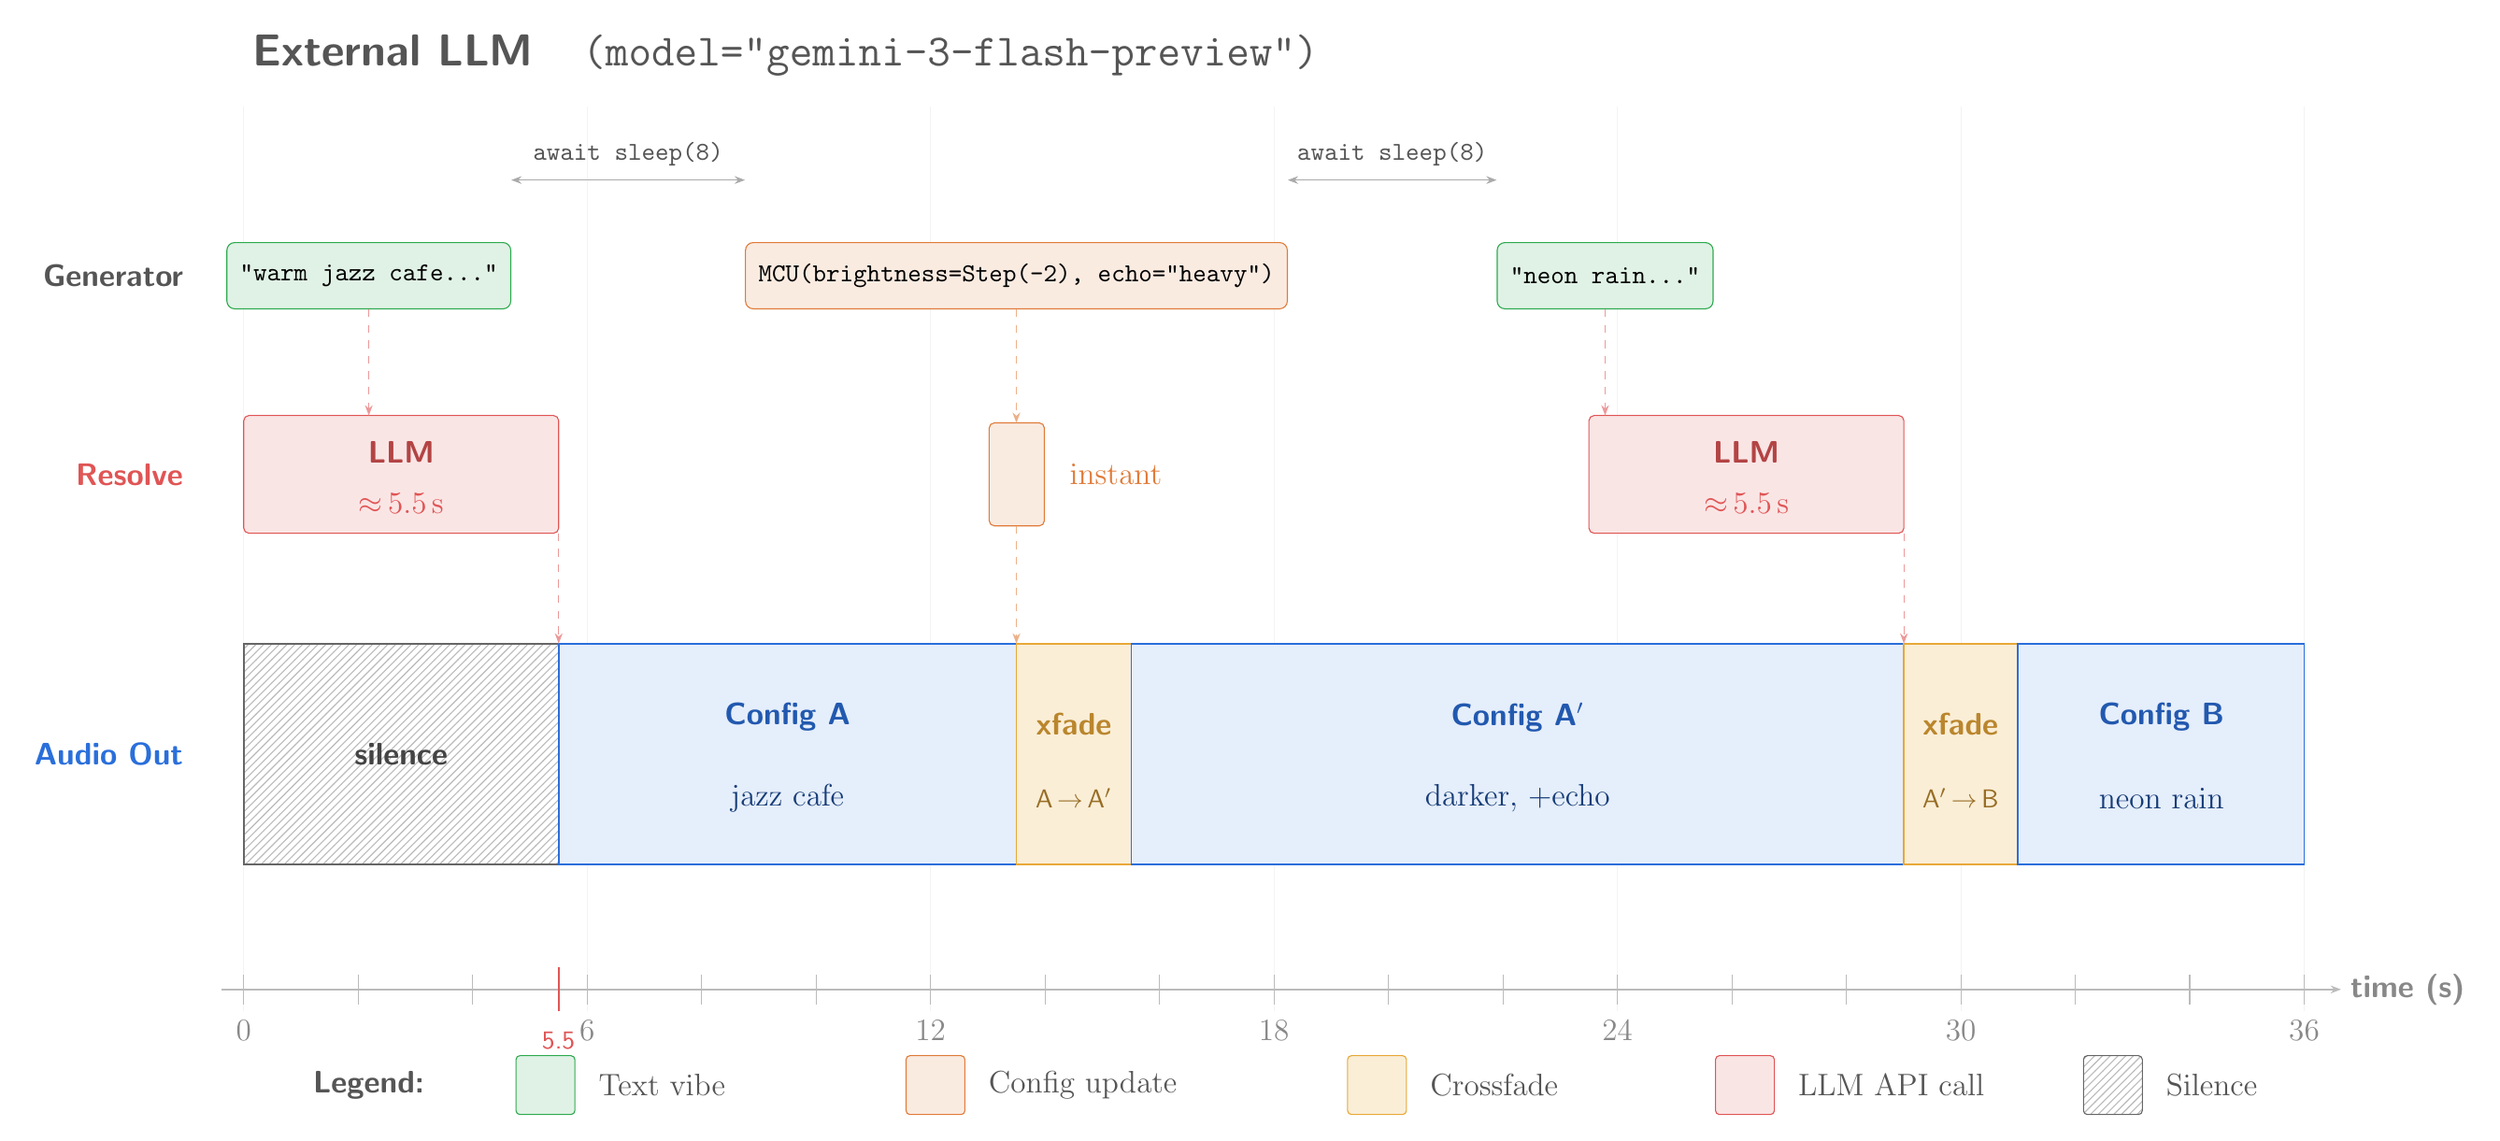
\begin{tikzpicture}[
    >={Stealth[length=4pt]},
    every node/.style={font=\large\sffamily},
]

%% x(t) = 3.5 + t * 28/36
%% t=0→3.50   t=5.5→7.78   t=13.5→14.00   t=15.5→15.56
%% t=23.5→21.78  t=29→26.06  t=31→27.61  t=36→31.50

% ── Title ──
\node[anchor=west, font=\LARGE\sffamily\bfseries, color=promptgray] at (3.5, 14.5)
    {External LLM ~~\texttt{(model="gemini-3-flash-preview")}};

% ── Row labels ──
\node[anchor=east, font=\large\sffamily\bfseries, color=promptgray] at (2.8, 11.5) {Generator};
\node[anchor=east, font=\large\sffamily\bfseries, color=llmred] at (2.8, 8.8) {Resolve};
\node[anchor=east, font=\large\sffamily\bfseries, color=audioblue] at (2.8, 5.0) {Audio Out};

% ── Light gridlines ──
\foreach \t in {0,6,12,18,24,30,36} {
    \pgfmathsetmacro{\xg}{3.5+\t*28/36}
    \draw[color=axisgray!18, line width=0.4pt] (\xg, 1.5) -- (\xg, 13.8);
}

% ═══════════════════════════════════════════
% GENERATOR ROW  (y = 11.5)
% ═══════════════════════════════════════════

\node[draw, rounded corners=3pt, fill=gengreen!15, draw=gengreen,
      minimum height=0.9cm, inner sep=5pt,
      font=\normalsize\ttfamily, align=center]
    (y1) at (5.2, 11.5) {"warm jazz cafe..."};

\node[draw, rounded corners=3pt, fill=updateorange!15, draw=updateorange,
      minimum height=0.9cm, inner sep=5pt,
      font=\normalsize\ttfamily, align=center]
    (y2) at (14.0, 11.5) {MCU(brightness=Step(-2), echo="heavy")};

\node[draw, rounded corners=3pt, fill=gengreen!15, draw=gengreen,
      minimum height=0.9cm, inner sep=5pt,
      font=\normalsize\ttfamily, align=center]
    (y3) at (22.0, 11.5) {"neon rain..."};

% ── Sleep arrows ──
\coordinate (sy) at (0, 12.8);
\draw[<->, thin, color=promptgray!50]
    (y1.east |- sy) -- (y2.west |- sy)
    node[midway, above=2pt, font=\normalsize\ttfamily, color=promptgray] {await sleep(8)};
\draw[<->, thin, color=promptgray!50]
    (y2.east |- sy) -- (y3.west |- sy)
    node[midway, above=2pt, font=\normalsize\ttfamily, color=promptgray] {await sleep(8)};

% ═══════════════════════════════════════════
% RESOLVE ROW  (y = 8.8, boxes 8.0–9.6)
% ═══════════════════════════════════════════

% r1: LLM call  t = 0 → 5.5  (x = 3.50 → 7.78)
\draw[fill=llmred!15, draw=llmred, rounded corners=2pt]
    (3.50, 8.0) rectangle (7.78, 9.6);
\node[color=llmred!80!black, font=\large\sffamily\bfseries] at (5.64, 9.1) {LLM};
\node[color=llmred, font=\large] at (5.64, 8.4) {${\approx}$\,5.5\,s};

% r2: instant MCU apply  t = 13.5  (x = 14.00)
\draw[fill=updateorange!15, draw=updateorange, rounded corners=2pt]
    (13.63, 8.1) rectangle (14.38, 9.5);
\node[color=updateorange, font=\large, anchor=west] at (14.6, 8.8) {instant};

% r3: LLM call  t = 23.5 → 29  (x = 21.78 → 26.06)
\draw[fill=llmred!15, draw=llmred, rounded corners=2pt]
    (21.78, 8.0) rectangle (26.06, 9.6);
\node[color=llmred!80!black, font=\large\sffamily\bfseries] at (23.92, 9.1) {LLM};
\node[color=llmred, font=\large] at (23.92, 8.4) {${\approx}$\,5.5\,s};

% gen → resolve arrows
\draw[->, dashed, color=llmred!60] (y1.south) -- (5.2, 9.6);
\draw[->, dashed, color=updateorange!60] (y2.south) -- (14.0, 9.5);
\draw[->, dashed, color=llmred!60] (y3.south) -- (22.0, 9.6);

% ═══════════════════════════════════════════
% AUDIO OUT ROW  (boxes 3.5–6.5)
% ═══════════════════════════════════════════

% Silence  t = 0 → 5.5  (x = 3.50 → 7.78)
\draw[pattern=north east lines, pattern color=waitgray!80,
      draw=waitgray!60!black, line width=0.6pt]
    (3.50, 3.5) rectangle (7.78, 6.5);
\node[font=\large\sffamily\bfseries, color=waitgray!40!black] at (5.64, 5.0) {silence};

% Config A "jazz cafe"  t = 5.5 → 13.5  (x = 7.78 → 14.00)
\draw[fill=audioblue!12, draw=audioblue, line width=0.6pt]
    (7.78, 3.5) rectangle (14.00, 6.5);
\node[font=\large\sffamily\bfseries, color=audioblue!80!black] at (10.89, 5.5) {Config A};
\node[font=\large, color=audioblue!55!black] at (10.89, 4.4) {jazz cafe};

% xfade A → A'   t = 13.5 → 15.5  (x = 14.00 → 15.56)
\draw[fill=crossfadeamber!20, draw=crossfadeamber, line width=0.6pt]
    (14.00, 3.5) rectangle (15.56, 6.5);
\node[font=\large\sffamily\bfseries, color=crossfadeamber!80!black] at (14.78, 5.4) {xfade};
\node[font=\normalsize\sffamily, color=crossfadeamber!65!black] at (14.78, 4.4) {A\,$\to$\,A$'$};

% Config A' "darker, +echo"  t = 15.5 → 29  (x = 15.56 → 26.06)
\draw[fill=audioblue!12, draw=audioblue, line width=0.6pt]
    (15.56, 3.5) rectangle (26.06, 6.5);
\node[font=\large\sffamily\bfseries, color=audioblue!80!black] at (20.81, 5.5) {Config A$'$};
\node[font=\large, color=audioblue!55!black] at (20.81, 4.4) {darker, +echo};

% xfade A' → B   t = 29 → 31  (x = 26.06 → 27.61)
\draw[fill=crossfadeamber!20, draw=crossfadeamber, line width=0.6pt]
    (26.06, 3.5) rectangle (27.61, 6.5);
\node[font=\large\sffamily\bfseries, color=crossfadeamber!80!black] at (26.83, 5.4) {xfade};
\node[font=\normalsize\sffamily, color=crossfadeamber!65!black] at (26.83, 4.4) {A$'$\,$\to$\,B};

% Config B "neon rain"  t = 31 → 36  (x = 27.61 → 31.50)
\draw[fill=audioblue!12, draw=audioblue, line width=0.6pt]
    (27.61, 3.5) rectangle (31.50, 6.5);
\node[font=\large\sffamily\bfseries, color=audioblue!80!black] at (29.56, 5.5) {Config B};
\node[font=\large, color=audioblue!55!black] at (29.56, 4.4) {neon rain};

% resolve → audio arrows
\draw[->, dashed, color=llmred!60] (7.78, 8.0) -- (7.78, 6.5);
\draw[->, dashed, color=updateorange!60] (14.00, 8.1) -- (14.00, 6.5);
\draw[->, dashed, color=llmred!60] (26.06, 8.0) -- (26.06, 6.5);

% ═══════════════════════════════════════════
% TIME AXIS
% ═══════════════════════════════════════════

\draw[->, thick, color=axisgray] (3.2, 1.8) -- (32.0, 1.8)
    node[right, font=\large\sffamily\bfseries, color=timegray] {time (s)};
\foreach \t in {0,2,...,36} {
    \pgfmathsetmacro{\xp}{3.5+\t*28/36}
    \draw[color=axisgray] (\xp, 1.6) -- (\xp, 2.0);
}
\foreach \t in {0,6,12,18,24,30,36} {
    \pgfmathsetmacro{\xp}{3.5+\t*28/36}
    \node[color=timegray, font=\large, anchor=north] at (\xp, 1.5) {\t};
}
% Special tick for t = 5.5  (first LLM resolve end → audio begins)
\pgfmathsetmacro{\xfirst}{3.5+5.5*28/36}
\draw[color=llmred, thick] (\xfirst, 1.5) -- (\xfirst, 2.1);
\node[color=llmred, anchor=north, font=\normalsize\sffamily] at (\xfirst, 1.35) {5.5};

% ═══════════════════════════════════════════
% LEGEND
% ═══════════════════════════════════════════

\node[font=\large\sffamily\bfseries, color=promptgray] at (5.2, 0.5) {Legend:};

\fill[gengreen!15, draw=gengreen, rounded corners=1.5pt] (7.2,0.1) rectangle (8.0,0.9);
\node[color=promptgray, font=\large, anchor=west] at (8.2, 0.5) {Text vibe};

\fill[updateorange!15, draw=updateorange, rounded corners=1.5pt] (12.5,0.1) rectangle (13.3,0.9);
\node[color=promptgray, font=\large, anchor=west] at (13.5, 0.5) {Config update};

\fill[crossfadeamber!20, draw=crossfadeamber, rounded corners=1.5pt] (18.5,0.1) rectangle (19.3,0.9);
\node[color=promptgray, font=\large, anchor=west] at (19.5, 0.5) {Crossfade};

\fill[llmred!15, draw=llmred, rounded corners=1.5pt] (23.5,0.1) rectangle (24.3,0.9);
\node[color=promptgray, font=\large, anchor=west] at (24.5, 0.5) {LLM API call};

\draw[pattern=north east lines, pattern color=waitgray!80,
      draw=waitgray!60!black, rounded corners=1.5pt] (28.5,0.1) rectangle (29.3,0.9);
\node[color=promptgray, font=\large, anchor=west] at (29.5, 0.5) {Silence};

\end{tikzpicture}
\end{document}
